This section presents previous work which inspired and layed the fundaments for this thesis. Relevant publication on topics related to this thesis will be presented in terms of methods and results. We focus on the fields of relational graph convolutions, graph encoders, and embedding based link prediction.

\subsection{Relational Graph Convolutions}
We define a graph as $G=(\mathcal{V}, \mathcal{E})$  with a set of nodes $\mathcal{V}$ and a set of edges $\mathcal{E}$. The set of edges, with each edge connecting node $x$ and $y$, is defined by $\left\{(x, y) \mid(x, y) \in \mathcal{V}^{2} \wedge x \neq y\right\}$ while the constrain $x \neq y$ prohibits self-connections or self-loops, which is optional depending on the graphs function. Moreover, nodes and edges can have features, which contribute additional information about the nodes and their connection. Using graph convolutions, we make use of these properties holding spectral information about their neighboring nodes and relations. The two main tasks to evaluate the performance of a neural network on graphs, are node classification and link prediction. The first is a classification problem where the model predicts the class of a node. For link prediction the model tries to distinguish the real triple in a set of corrupted triples. A more in-depth explanation follows later on in chapter \ref{sec:mthods}.

% Present the relational graph convolution model paper by Kipf and maybe others
In Kipf \textit{et al.} first paper on graph convolutions \cite{kipf_semi-supervised_2017} a novel Graph Convolution Network (GCN) for semi-supervised classification is introduced. The model takes as input the adjacency and optionally a feature matrix of the graph and predicts the  This method acts directly on the graph structure and shows to be linearly scalable with the number of nodes. While the authors compare different propagation models for the graph convolutions, their propagating rule using a first-order approximation of spectral graph convolutions, outperforms all other implementations. The so-called renormalization trick normalized the adjacency matrix and adds it to an identity matrix of same size. This keeps the eigenvalues in a range between $[0,2]$ which again leads to a stable training, avoiding numerical instabilities and vanishing gradients during learning. Additionally the feature information of neighboring nodes is propagated in every layer what shows improvement in comparison to earlier methods, where only label information is aggregated.
Kipf and Welling perform node classification on the three citation-network datasets, Citeseer, Cora and Pubmed as well as on the KG dataset NELL. In all classification tasks, their results outperform other recently proposed methods in this field and proves to be computationally more efficient than its competition. For more details on the implementation of graph convolutions we refer to the background section \ref{ssec:gcn}. 


% node classification
% on datasets: citation network Citeseer Cora Pubmed and knowledge graph  NELL


% Kipfs second paper 
In their publication \textit{Modeling Relational Data with Graph Convolutional Networks} Schlichtkrull \textit{et al.} propose a relational graph convolutional network (RGCN) and evaluate it on link prediction on the FB15K-237 and WN18 dataset and node classification on the AIFB, MUTAG, BGS and AM datasets \cite{gangemi_modeling_2018}. While the RGCN, with its encoder properties, is used by itself as node classifier, yet for link prediction it is coupled with a DistMult model acting as decoder which scores triples encoded by the RGCN see \ref{fig:RGCN}. More details on DistMult can be found in \ref{ssec:embedlp}.

\begin{figure}[h]
    \centering
    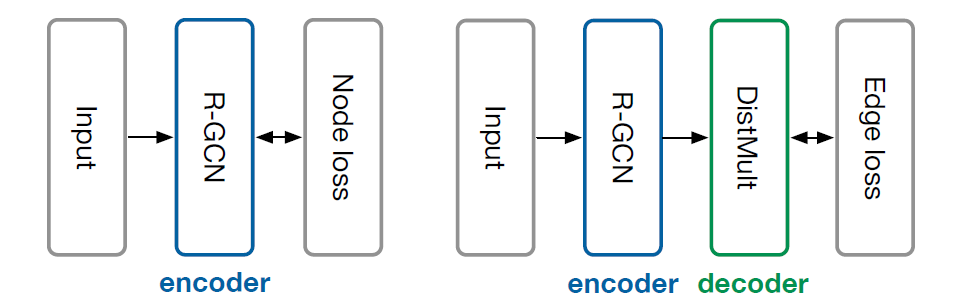
\includegraphics[width=0.55\textwidth]{data/images/RGCN.png}
    \caption{RGCN pipeline for node classification and link prediction experiments. The first pipeline only uses an encoder to classify the input nodes. The second pipeline additionally uses a decoder to score the input and predict the correct link, Source \cite{gangemi_modeling_2018}.}
    \label{fig:RGCN}
\end{figure}

The RGCN works on graphs stored as dense triples, creating a hidden state for head and tail of each triple. A novel message passing network is layer-wise propagated with the hidden states of the entities. As regularization the authors propose a \textit{basis-} and \textit{blockwise} decomposition. while the first  aims at an effective weight sharing between different relation types, the second  can be seen as a sparsity constraint on the relation type's weight. The model outperforms embedding based model on the link prediction task on the FB15K-237 dataset and scores competitive on the WN18 dataset. In the node classification task, the model sets state of the art results on the datasets AIFB and AM, while scoring competitive on the remaining. The authors conclude, that the model has difficulties encoding higher-degree hub nodes on datasets with many entities and low amount of classes.


\subsection{Graph VAE}
% Present different papers with graph VAEs
We have seen how graph convolutional neural networks can be combined to a encoder-decoder architecture, resulting in a generative model suitable for unsupervised learning. We will present three recent publications with different methods and use cases of a graph generative model, in particular a VAE.

% Kipfs VGAE
In yet another publication of Kipf \textit{et al.} the Variational Graph Autoencoder (VGAE) is introduced, a framework for unsupervised learning on graph-structured data \cite{kipf_variational_2016}. This generative model uses a GCN as encoder and a simple inner product module as decoder. Similar to th GCN the VGAE incorporates node features, what significantly improves its performance on link prediction tasks compared to related models. The VGAE uses a two-layer GCN to encode the mean and the logvariance for the stochastic module to sample the latent space representation. The activation of the inner product of this latent vector yields the reconstruction of the adjacency matrix. Figure \ref{fig:kipfGVAE} shows how the model learns to represent the underlying data structure by grouping the Gaussian latent representations of the datapoints according to their class, without these labels being provided to the model during training.

\begin{figure}[h]
    \centering
    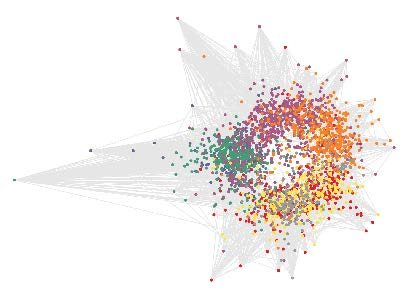
\includegraphics[width=0.5\textwidth]{data/images/KipGVAE.jpg}
    \caption{Colorized visualization of the latent representation of the VGAE trained on the Core citation network with colors differentiating document classes and gray links indicating citations. This shows that the model implies and featurizes the document classes, without them being provided during training. Source \cite{kipf_variational_2016}}
    \label{fig:kipfGVAE}
\end{figure}

The VGAE with added features outperforms state of the art models in the task of link prediction on the datasets Cora, Citeseer and Pubmed. The authors point out, that a Gaussian prior might be a poor choice combined with the inner-product decoder.

While citation networks represent basic graph structures, work has also been done on more complex KGs.
Simonovsky \textit{et al.} introduce the GraphVAE, a generative model which outputs a probabilistic fully-connected graph of a predefined maximum size
in a one-shot approach \cite{simonovsky_graphvae_2018}. The model includes a standard graph matching algorithm to align the predicted graph to the ground truth. In contrast to the previously presented publications, the input to this model is a threefold and sparse graph, defined as $G=(A, E, F)$ with $A$ being the adjacency matrix, $E$ the edge attribute matrix and $F$ the node attribute matrix, with $E$ and $F$ being one-hot encoded. Considering that this method lays the foundation for this thesis, we will adopt this notation for our own methods in \ref{sec:mthods}. Figure \ref{fig:graphvaefull} shows the architecture of the GraphVAE. The encoder is a feed forward network with edge-conditioned graph convolutions. After the convolutions the result is flattened and conditioned on the node labels $y$. A simple neural network then encodes the stochastic latent space, as we know it from previous works. The decoder is again conditioned on the node labels $y$ and in form of a fully-connected neural network reconstructs the latent representation to the graph prediction. The threefold decoder output is matched with the target using graph matching algorithm, which we will discuss further in \ref{ssec:graphmatch}. The best matching permutation is then used for the reconstruction loss term of the GraphVAE. It should be noted, that the size of the target and prediction graph do not necessarily have to match. While this approach seems promising, the maximum graph size is limited to a node count of $~100$ by computational memory requirements.

\begin{figure}[h]
    \centering
    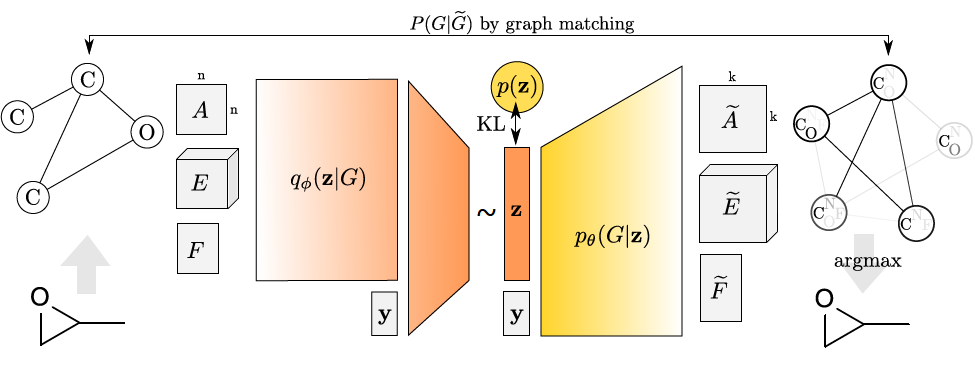
\includegraphics[width=0.9\textwidth]{data/images/GraphVAEfull.png}
    \caption{Model architecture of the GraphVAE. The target graph with $n$ nodes is encoded and conditioned on the node labels $y$. The KL divergence ensures a Gaussian prior to the decoder, which reconstructs the latent representation to a graph with $k$ nodes. Target and prediction graphs are matched and permuted before the reconstruction loss. To sample, the argmax is taken directly from the prediction. Source \cite{simonovsky_graphvae_2018}.}
    \label{fig:graphvaefull}
\end{figure}

The model is trained on the QM9 dataset, containing the graph structure of 134k organic molecules with experiments on latent space dimension in the range of $[20,80]$. On the free generation task, about $50\%$ of the generated molecules are chemically valid and thereof remarkably $60\%$ are not included in the trainings dataset. When testing the model for robustness, it showed little disturbance when adding Gaussian noise to the input graph $G$. The authors conclude that the problem of generating graphs
from a continuous embedding was addressed successfully and that the GraphVAE performs better on small molecules, thus worse on larger graphs.


In a little sidestep, we present the idea of supervised graph generation in an autoregressive fashion by Belli \textit{et al.} and their publication \textit{Image-Conditioned Graph Generation for Road Network Extraction} \cite{belli_image-conditioned_2019}. While we will focus on the generative model, their contribution ranges wider, namely the introduction of the graph-based roadmap dataset \textit{Toulouse Road Network} and the task specific distance metric \textit{StreetMover}. The authors propose the Generative Graph Transformer (GGT) a deep autoregressive model that makes use of attention mechanisms on images, to tackle the challenging task of road network extraction from image data. The GGT has a encoder-decoder architecture, with a CNN as encoder, taking the grayscale image as input signal and predicting a conditioning vector. The decoder is a self-attentive transformer, which takes as input the encoded condition vector and a hidden representation of the adjacency matrix $A$ and feature vector $X$ of the previous step. The adjacency matrix here indicates the links between steps and the features are normalized coordinates. A multi-head operator outputs the hidden representation of $A$ and $X$ which finally are decoded by a MLP to the graph representation. For the fist step, a empty hidden representation is fed into the decoder. The model terminates the recurrent graph generation by predicting a end-of-sequence token, which signalizes the end of the graph. During learning, the generated graphs are matched to the target graphs using the \textit{StreetMover} metric, based on the Sinkhorn distance. The authors attribute \textit{StreetMover} as a scalable, efficient and permutation-invariant metric for graph comparison. The successful results of the experiments performed, show that this novel approach is suitable for the task of road network extraction and could yield similar success in graph generation task of different fields.
While this publication does not directly align with the previously presented work, we find it of added value to present alternative approaches on our topic.

% \begin{itemize}
%     \item Belli recurrent VAE
%     \item GraphVAE paper
%     \item Variational Graph Auto-Encoders
% \end{itemize}


\subsection{Embedding Based Link Prediction}
\label{ssec:embedlp}
Finalizing this chapter, we will look at embedding based methods on KGs. This approach was inspired by the success of word-embeddings in the field of NLP. Compared to the previously presented research, embedding models have a much simpler architecture and can be trained computationally very efficiently on large graphs. Embedding based models can only operate on simple triples, meaning a KG is represented as a set of triples with indices pointing to the unique entity and relation in the graph. In disregard of their simplicity, they achieve great results on relational prediction tasks such as link prediction. In particular, this means to rank a correct triple the highest between a set of corrupted triples. In order to generate corrupt triples, each triple from the test set is modified by replacing the head or tail with all remaining entities occurring in the KG. Link prediction will be explained in more detail in \ref{sec:mthods}. 


Already in 2013 Bordes \textit{et al.} introduced in their paper \textit{Translating Embeddings for Modeling Multi-relational Data} the low-dimensional embedding model TransE \cite{bordes_translating_2013}. The core idea of this model is that relations can be represented as translations in the embedding space. Entities are encoded to a low-dimension embedding space and the relation is represented as vector between the head and tail entity. The assumption is, that correct triples have a lower norm of the relational vector than corrupted triples, thus, the distance between head and tail entity in embedding space is less. The loss function for learning of the model takes a set of corrupted triples for every triples in the training set and subtracts the translation vector of the corrupted triple in embedding space from the translation vector of the correct triple with added margin. To minimize the loss, the model has to place entities of correct triples closer together in embedding space. We think of a triple as $(s,r,o)$ and the bold notation as its embedded representation, $d()$ the distance measure, $\gamma$ the positive margin and $S$ and $S^{\prime}$ as sets of correct and corrupt triples, the loss function of TransE is 

\begin{equation}
    \mathcal{L}=\sum_{S} \sum_{S^{\prime}} \left[\gamma+d(\boldsymbol{s}+\boldsymbol{r}, \boldsymbol{o})-d\left(\boldsymbol{s}^{\prime}+\boldsymbol{r}, \boldsymbol{o}^{\prime}\right)\right]
\end{equation}

The model is trained on the two KGs Freebase and Wordnet, which will also be the source for the datasets used in this thesis. TransE's link prediction results on both head and tail outperformed other competing methods of the time, such as RESCAL \cite{nickel_three-way_nodate}.

In 2015, Yang \textit{et al.} proposed a similar, yet better performing KG embedding method \cite{yang_embedding_2015}. Their model DistMult captures relational semantics by matrix multiplication of the embedded entity representation and uses a bilinear learning objective. The main difference to TransE is the bilinear scoring function $d_{r}^{b}()$, where bilinear denotes the score invariance of swapping head and tail entity. For the embedding space representation of subject and object $\boldsymbol{s}$ and $\boldsymbol{o}$ and a diagonal matrix $\mathbf{M}_{r} \in \mathbb{R}^{n \times n}$ as embedding of $r$, the scoring function is

\begin{equation}
    d_{r}^{b}\left(\boldsymbol{s}, \boldsymbol{o}\right)=\boldsymbol{s}^{T} \mathbf{M}_{r} \boldsymbol{o}
    \label{eq2:distmult}
\end{equation}

The publication goes on to explore the options of embedding based rule extraction from KGs. Concluding, the authors state that that embeddings learned from the bilinear objective not only outperform the state of the art in link prediction but can also capture compositional semantics of relations and extract Horn rules using compositional reasoning.


In a more recent publication by Ruffinelli et al. re-trained outdated KG embedding models such as TransE and DistMult with state of the art techniques in deep learning. The authors start by pointing out the similarities and differences of most models. While all methods share the same embedding approach, they differ in their scoring function and their original hyperparameter search. The authors perform a quasi-random hyperparameter search on the five models RESCAL, TransE, DistMult, ComplEx and ConvE using the two datasets FB15K-237 and WN18. For evaluation the MRR and Hits@$10$ are used. Since these metrics and datasets will be used later on in our research, they are explained in \ref{ssec5:data}(datasets) and \ref{ssec4:lpmetrics}(metrics). The tuned models report a higher MRR score of up to $24\%$ compared to their first reported performance. The authors conclude that simple KG embedding methods can show strong performance when trained with state-of-the-art techniques and score competitive to or even outperforme more recent architectures. The improved model configurations were found by exploring relatively few random samples from a large hyperparameter space. 

% Graph Embeddings\\
% TransE represents entities in in low-dimensional embedding. The relationships between entities are represented by the vector between two entities \cite{bordes_translating_2013}.
% (How are different relation between the same entities represented?)

% OntoUSP\\
% This method learns a hierarchical structure to better represent the relations between entities in embedding space.
